\documentclass{amsbook}

\usepackage[
    a5paper,
    margin=28mm,
    marginparwidth=20mm,
    marginparsep=3mm
]{geometry}

#PACKAGE_CODE

\title{The First Book. Lucifer in Starlight}

\begin{document}
\frontmatter
\renewcommand\thefootnote{{}}
\maketitle

\thispagestyle{empty}
\topskip0pt
\vspace*{\fill}
\noindent {\it How you are fallen from heaven, Lucifer, son of the morning. How you are cut down to the ground, you who laid nations low. You said in your heart, I will ascend into heaven; I will exalt my throne above the stars of God; I will ascend above the heights of the clouds; I will make myself like the Most High. But you are brought down to hell, to the depths of the pit...}
\vspace*{\fill}
\clearpage

\tableofcontents

\thispagestyle{empty}
\topskip0pt
\vspace*{\fill}
{\centering
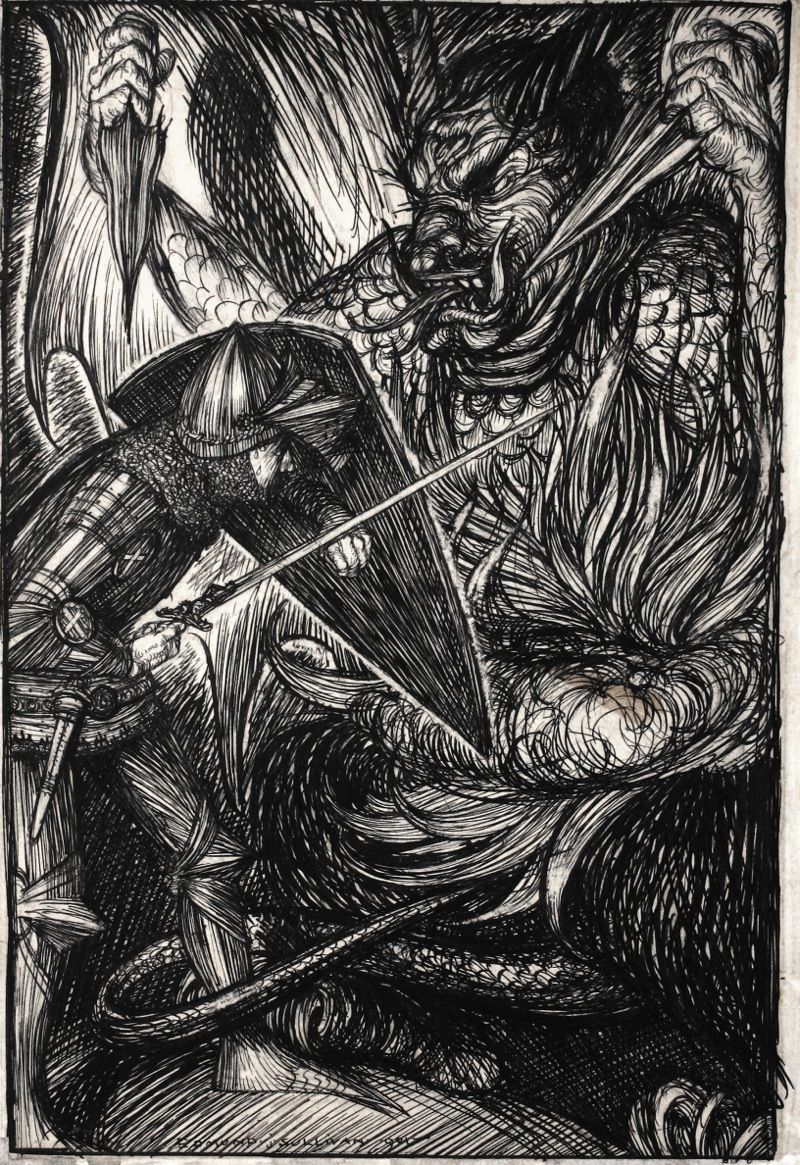
\includegraphics[width=\textwidth]{images/placeholder_image.jpg}}
\vspace*{\fill}
\clearpage

\thispagestyle{empty}
\topskip0pt
\vspace*{\fill}
\noindent {\sc Argument:} {\itshape How the two lovers from \emph{William's Farewell}, having suffered an unrecoverable loss, wandered across the country; and of the strange things that befell them on their way.}
\vspace*{\fill}
\clearpage

\thispagestyle{empty}
\topskip0pt
\vspace*{\fill}
{\centering
\includegraphics[width=\textwidth]{#AUTUMNAL_IMAGE}}
\vspace*{\fill}
\clearpage

\mainmatter

\chapter{Autumnal}

\renewcommand{\poemone}{
    #AUTUMNAL_POEM_1
}
\renewcommand{\poemtwo}{
    #AUTUMNAL_POEM_2
}
\renewcommand{\poemthree}{
    #AUTUMNAL_PRAYER
}
\initprintpoems
#AUTUMNAL_PROSE
\clearpage

\thispagestyle{empty}
\topskip0pt
\vspace*{\fill}
{\centering
\includegraphics[width=\textwidth]{#HIBERNAL_IMAGE}}
\vspace*{\fill}
\clearpage

\chapter{Hibernal}

\renewcommand{\poemone}{
    #HIBERNAL_POEM_1
}
\renewcommand{\poemtwo}{
    #HIBERNAL_POEM_2
}
\renewcommand{\poemthree}{
    #HIBERNAL_PRAYER
}
\initprintpoems

#HIBERNAL_PROSE
\clearpage

\thispagestyle{empty}
\topskip0pt
\vspace*{\fill}
{\centering
\includegraphics[width=\textwidth]{#VERNAL_IMAGE}}
\vspace*{\fill}
\clearpage

\chapter{Vernal}

\renewcommand{\poemone}{
    #VERNAL_POEM_1
}
\renewcommand{\poemtwo}{
    #VERNAL_POEM_2
}
\renewcommand{\poemthree}{
    #VERNAL_PRAYER
}
\initprintpoems

#VERNAL_PROSE
\clearpage

\thispagestyle{empty}
\topskip0pt
\vspace*{\fill}
{\centering
\includegraphics[width=\textwidth]{#AESTIVAL_IMAGE}}
\vspace*{\fill}
\clearpage

\chapter{Aestival}

\renewcommand{\poemone}{
    #AESTIVAL_POEM_1
}
\renewcommand{\poemtwo}{
    #AESTIVAL_POEM_2
}
\renewcommand{\poemthree}{
    #AESTIVAL_POEM_3
}
\initprintpoems

#AESTIVAL_PROSE

\bigskip
\bigskip
\begin{center}
    \textsc{End of the First Book}
\end{center}

\end{document}
